\aufgabe 1

\paragraph{a)}\mbox{} \\

\begin{figure}[H] 
	\centering 
	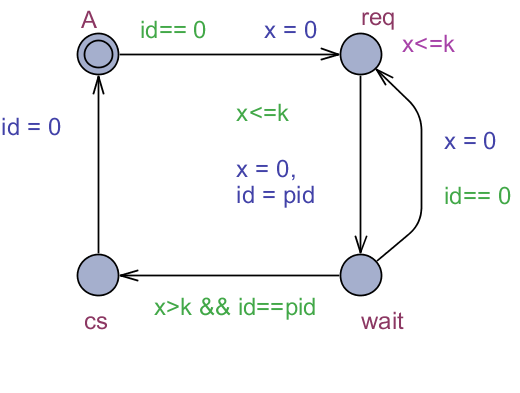
\includegraphics[width=0.5\textwidth]{./UPAAAL_Screens/Aufgabe1a}
	\caption[Aufgabe 1a)]{Geladenes Programm fisher.xml}    
\end{figure}


\paragraph{b)}\mbox{} \\

\begin{figure}[H] 
	\centering 
	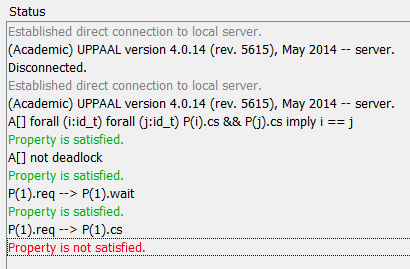
\includegraphics[width=0.5\textwidth]{./UPAAAL_Screens/Aufgabe1b}
	\caption[Aufgabe 1b)]{Ergebnisse der Verifizierung der Properties}    
\end{figure}

\newpage

\paragraph{c)}\mbox{} \\

\begin{figure}[H] 
	\centering 
	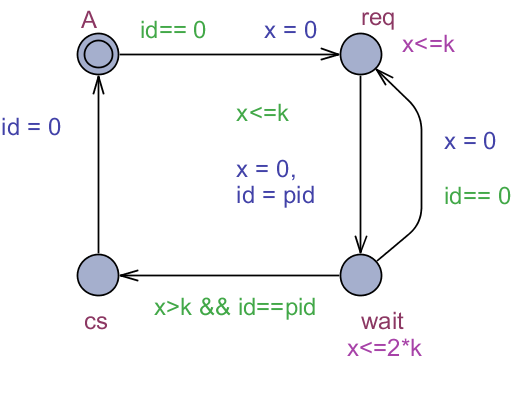
\includegraphics[width=0.5\textwidth]{./UPAAAL_Screens/Aufgabe1c_Invariante}
	\caption[Aufgabe 1c)]{Zeitautomat mit hinzugefügter Invariante in $wait$}    
\end{figure}

\begin{figure}[H] 
	\centering 
	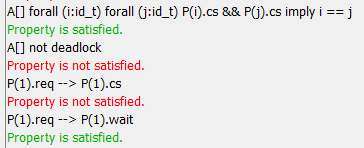
\includegraphics[width=0.5\textwidth]{./UPAAAL_Screens/Aufgabe1c_Testlaeufe}
	\caption[Aufgabe 1c)]{Ergebnisse der Verifizierung der Properties mit hinzugefügter Invariante in $wait$}    
\end{figure}

Im Vergleich zu Teilaufgabe b) enthält das Modell durch Hinzunahme der Invariante $x\leq2*k$ im Zustand $wait$ einen Deadlock und erfüllt somit nicht die Eigenschaft $A[] \text{not deadlock}$. Der Deadlock entsteht dabei folgendermaßen: \\

Der erste Prozess $P(1)$ betritt zunächst den Zustand $wait$. Aufgrund des Guards $x>k$ muss Zeit verstreichen. Als nächstes spring der zweite Prozess $P(2)$ in den $wait$-Zustand. Dabei befindet sich die Clock $x \in \left[2,4\right]$. $P(1)$ müsste nun aufgrund der neuen Invariante den Zustand verlassen, da die für den Zustand $cs$ freigegebene $id == 2$ und $pid ==1$ ist,  wird der Guard $id == pid$ nicht erfüllt. Weil $P(1)$ somit nicht auf einen anderen Zustand wechseln und $id$ nicht auf 0 zurückgesetzt werden kann, kommt es zu einem Deadlock. \\

Aufgrund dessen kann ebenso die Verifizierung $P(1).\text{req} --> P(1).\text{cs}$ nicht erfüllt werden.  

\paragraph{d)}\mbox{} \\

\begin{figure}[H] 
	\centering 
	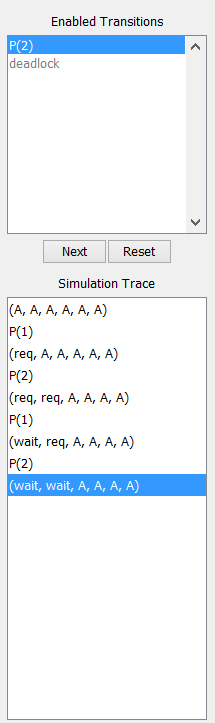
\includegraphics[height=0.4\textheight]{./UPAAAL_Screens/Aufgabe1d_Trace}
	\caption[Aufgabe 1d)]{Diagnostic Trace des Deadlocks des Automaten aus Teilaufgabe 1c)}    
\end{figure}

\begin{figure}[H] 
	\centering 
	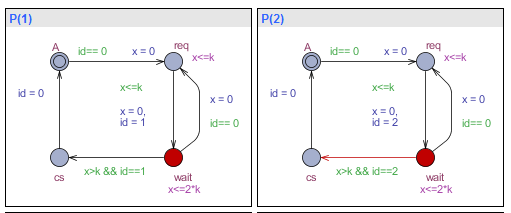
\includegraphics[width=0.5\textwidth]{./UPAAAL_Screens/Aufgabe1d_TraceGraph}
	\caption[Aufgabe 1d)]{Zugehörige Deadlocks zum oben angegebenem Trace}    
\end{figure}
